\documentclass[10pt]{article}

% Margins and layout
\usepackage[left=0.75in,right=0.75in,top=0.8in,bottom=0.8in]{geometry}

% Encoding
\usepackage[T1]{fontenc}
\usepackage[utf8]{inputenc}

% Font package
\usepackage{times}

% No paragraph indent, less space between paragraphs
\setlength{\parindent}{0pt}
\setlength{\parskip}{0.7em}

% Page number in footer
\usepackage{fancyhdr}
\pagestyle{fancy}
\fancyhf{}
\cfoot{\thepage}
\renewcommand{\headrulewidth}{0pt}
\renewcommand{\footrulewidth}{0pt}

% Needed for [H] placement of figures
\usepackage{float}

% Graphics
\usepackage{graphicx}

% Optimize table layouts
\usepackage{booktabs}
\usepackage{array}
\usepackage{tabularx}

% Make links compact
\usepackage[colorlinks=true,linkcolor=blue,citecolor=blue]{hyperref}

% Math and bibliography
\usepackage[numbers]{natbib}
\usepackage{amsmath,amssymb}

% Make lists more compact
\usepackage{enumitem}
\setlist{noitemsep,topsep=2pt,parsep=0pt,partopsep=0pt}

% Column separation for two-column sections if needed
\usepackage{multicol}
\setlength{\columnsep}{0.5cm}

% More compact figure captions
\usepackage[font=small,labelfont=bf]{caption}

% More compact section titles
\usepackage{titlesec}
\titlespacing*{\section}{0pt}{1em}{0.5em}
\titlespacing*{\subsection}{0pt}{0.8em}{0.3em}
\titlespacing*{\subsubsection}{0pt}{0.6em}{0.2em}

\title{REPLACE WITH PAPER TITLE}
\author{Diyan Gao, Anish Chandra, Linglong Meng}
\date{April 2025}

\begin{document}

\maketitle

\section{Introduction}

This study investigates how Large Language Model (LLM) agents can autonomously learn to use external memory systems when faced with sequential reasoning tasks. Prior research on memory-augmented agents has often relied on predefined memory architectures or hard-coded usage patterns, limiting the adaptability of such systems. Here, we explore a more flexible approach: equipping agents with multiple memory systems, minimal instructions, and allowing them to develop memory usage strategies that align with their objectives.

To create a controlled yet scalable environment for this exploration, we implement a self-play setup in TicTacToe. The environment ranges from the familiar $3 \times 3$ board to larger, more complex $6 \times 6$ and $9 \times 9$ boards. This scaling of the state space allows us to examine how memory usage strategies evolve with task complexity, and how different memory architectures support decision-making under varying conditions.

Our agents—built on the Cognitive Language Agent (CLA) framework—share the same underlying architecture, pairing OpenAI's GPT-4o-mini with external memory modules. However, they differ solely in their \textbf{prompt framing}: Agent A maximizes win rate without cost considerations, while Agent B balances win rate against token efficiency, explicitly guided by a win–token tradeoff formula and repeated reminders of memory costs. This setup isolates prompt-level guidance as the primary factor shaping agent behavior, holding architecture and task environment constant.

The agents interact with three complementary memory modalities: \textbf{GraphMemory} for structured, relational data; \textbf{VectorMemory} for similarity-based retrieval in embedding space; and \textbf{SemanticMemory} for conceptual storage (though SemanticMemory remains a placeholder in this work and is not evaluated due to time constraints). Through two experimental regimes—\textbf{constrained}, where agents are restricted to a single memory type, and \textbf{adaptive}, where agents can freely choose among available memory systems—we systematically evaluate how these architectures affect learning trajectories, scalability, and emergent strategies. Detailed logging of every memory call, token expenditure, and action rationale enables us to map memory usage patterns to agent performance.

Our results reveal significant differences in how agents deploy memory across architectures and objectives, offering new insights into designing adaptive, goal-driven memory systems for LLM agents operating in increasingly complex environments.

\section{Methods}

We evaluate our agents in a self-play TicTacToe environment, where two agents face off across varying board sizes ($3 \times 3$, $6 \times 6$, and $9 \times 9$). This setup offers a structured yet scalable domain for testing sequential reasoning, as the expansion of the board dramatically increases the state space and planning depth required for optimal play. The simplicity of TicTacToe facilitates clear interpretations of agent behavior, while the scaling provides a mechanism to probe memory demands under different levels of complexity.

Both agents in each game share a common architecture. Each is composed of a GPT-4o-mini core paired with external memory modules. The Cognitive Language Agent (CLA) framework guides this setup, combining a powerful language model with structured memory systems \cite{sumers2024cognitivearchitectureslanguageagents}. The key difference between the two agents lies in their objectives and prompt design. Agent A focuses on maximizing win rate without regard for efficiency, while Agent B balances winning with minimizing token use.

The agents interact with two primary types of external memory. \textbf{GraphMemory} organizes experiences as nodes and transitions, encoding structured relationships between game states. This architecture supports relational reasoning and enables the retrieval of paths through the game space. \textbf{VectorMemory}, by contrast, encodes states into fixed-dimensional embeddings via a simple autoencoder, facilitating similarity-based retrieval. This approach is better suited for pattern matching and generalization across loosely structured state spaces. While \textbf{SemanticMemory} is conceptually designed to handle higher-level strategy representations, it remains untested in this iteration and is excluded from the reported experiments, we will look into chances of investing in it even after the final report.

We conduct two main types of experiments. In the \textbf{constrained} setting, agents are restricted to a single memory type throughout a series of games. This isolates the effect of each architecture on performance, token usage, and memory behavior. In the \textbf{adaptive} setting, agents have access to all memory types and can choose which to use at each decision point. This allows us to probe whether agents can learn not only when to use memory, but which memory type to use depending on context.

For \textbf{baseline comparisons}, we evaluate memory-augmented agents against their no-memory counterparts. Each memory-enabled agent (Agent A or Agent B) is matched against an identical agent with memory modules disabled, isolating the effect of memory itself. Additionally, we compare Agent A without memory against Agent B without memory, providing a baseline for understanding the inherent effects of token efficiency tradeoffs without memory augmentation.

To ensure fair comparisons across agents, all experiments reset memory at the start of each experiment (spanning 15 or 30 games depending on the design). This design allows memory to persist across games within the same experiment, enabling us to examine whether LLM agents can leverage cross-game experiences to refine their strategies. By allowing memory carryover within experiments but not across them, we focus our analysis on within-experiment memory dynamics and learning behaviors. Throughout, we log token usage, memory calls, and agent rationales at each turn, enabling fine-grained insights into how memory strategies evolve under different conditions.

\subsection{The Agent: Agent A vs. Agent B}
Our agents are built on the Cognitive Language Agent (CLA) framework, combining a large language model (LLM) core with external memory systems to support long-term reasoning and strategy development \cite{sumers2024cognitivearchitectureslanguageagents}. The LLM used in this study is OpenAI's GPT-4o-mini, chosen for its balance between computational efficiency and expressive power. This architecture allows agents to integrate sequential experiences across games via external memory, while relying on the LLM for flexible reasoning.

\paragraph{Design Differences.}
Both agents share the same architecture and memory access mechanisms, but differ critically in their prompt framing and cost modeling, which jointly shape their memory usage strategies. While both agents are assigned the same explicit objective—maximize win rate while minimizing token usage—the underlying tradeoff parameter ($\lambda$) and prompt guidance diverge:

Agent A receives system prompts that focus purely on win rate maximization, with no mention of token costs or any tradeoff parameter. In effect, Agent A operates as if $\lambda = 0$.

Agent B, in contrast, is explicitly reminded of the token costs associated with memory operations. Its prompt specifies a concrete optimization formula:
$$
\text{maximize: win rate} - \lambda \times \text{token cost}
$$
where $\lambda$ governs the balance between winning and efficiency.

This design isolates the influence of implicit prompt guidance and cost sensitivity modeling. Although both agents nominally share the same objective in the system (maximize win rate while minimizing token use), Agent B receives additional framing and a defined $\lambda$, which lead it to adopt more conservative memory strategies. This subtle but crucial difference allows us to explore how LLM agents internalize tradeoffs between performance and resource efficiency.

\paragraph{Hypothesized Behavior.} This design allows us to investigate how \textbf{subtle variations in prompt framing}---rather than differing objective functions---shape emergent behaviors. We hypothesize that, even under a shared formal objective, agents will exhibit distinct memory usage patterns based on the implicit guidance embedded in their prompts:
\begin{itemize}[leftmargin=*,nosep]
    \item Agent A, unburdened by efficiency concerns, is expected to adopt a more \textbf{aggressive memory strategy}
    \item Agent B is encouraged toward \textbf{selective, resource-conscious behaviors}
\end{itemize}

\paragraph{Baseline Comparisons.}
To rigorously assess the influence of memory augmentation, we implement a structured set of baseline comparisons. For each agent type (Agent A and Agent B), we compare the performance of a memory-augmented agent against an identical agent with external memory modules fully disabled. These no-memory agents retain the same GPT-4o-mini core and system prompts as their memory-augmented counterparts, ensuring that any performance difference can be attributed solely to the presence or absence of external memory systems. This design isolates the marginal effect of memory under fixed agent configurations.

Beyond within-agent comparisons, we also conduct cross-agent baseline tests. Specifically, we compare \textbf{Agent A without memory} to \textbf{Agent B without memory}. This pairing enables us to evaluate whether the token-efficiency framing in Agent B's prompt affects decision quality even in the absence of memory. Since both agents share the same underlying model and are stripped of memory access, any performance divergence here reflects the impact of prompt-induced behavior under resource constraints.

In total, this baseline design enables three key contrasts:
\begin{enumerate}[leftmargin=*,nosep]
    \item \textbf{Memory-enabled vs. no-memory agents (within agent type)}: Isolating the performance lift due to memory architectures.
    \item \textbf{Agent A no-memory vs. Agent B no-memory}: Assessing token efficiency tradeoff effects in a memory-free setting.
\end{enumerate}

Experiments are conducted across two board sizes—$3 \times 3$ and $9 \times 9$—to capture the effects of task complexity on baseline dynamics. Each experimental condition runs for 15 games per pairing, balancing computational cost with statistical robustness. All baseline agents operate under the same memory-reset logic as their memory-augmented counterparts, ensuring comparability in experimental conditions.

\subsection{Memory Module Architecture}

To study the role of external memory in agent reasoning, we implement two complementary memory systems—\textbf{VectorMemory} and \textbf{GraphMemory}—each accessible via \verb|store| and \verb|retrieve| function bindings. These systems enable agents to record and recall experiences across game states, shaping their decision-making processes over time.

\paragraph{VectorMemory.} 
VectorMemory encodes each game state into a fixed-dimensional embedding, supporting similarity-based retrieval. Specifically, each $3 \times 3$ board is flattened into a 9-dimensional vector, which is passed through a simple autoencoder. The encoder compresses this input into a 6-dimensional latent space using a single linear layer with ReLU activation, while the decoder reconstructs the original input. Retrieval queries the memory with a current board state and returns the most similar stored vectors based on cosine similarity, facilitating pattern matching across structurally similar states. Metadata associated with each vectorized entry enables the agent to store strategic annotations alongside board configurations.

\paragraph{GraphMemory.}
GraphMemory organizes experiences as a directed graph, where each node represents a unique game state and edges encode transitions between states (moves). When an agent issues a retrieval query, it receives all immediate successor states and their metadata, providing a local relational context. This structure supports reasoning over sequential transitions and allows the agent to revisit past game paths.

\paragraph{Constrained vs. Adaptive Memory Use.}
We evaluate memory usage under two regimes. In \textbf{constrained} settings, agents are restricted to a single memory type (either GraphMemory or VectorMemory), enforced via system prompts and runtime checks that block disallowed memory operations. This isolates the impact of each memory architecture. In \textbf{adaptive} settings, agents have access to all available memory types and can choose which to use at each turn, enabling the exploration of emergent memory selection strategies.

\paragraph{Schema Updates.} 
In addition to \texttt{store} and \texttt{retrieve}, our memory systems expose a meta-memory operation, \texttt{updateSchema}, which allows agents to modify the structure or metadata schema of stored entries. While this functionality is implemented at the memory management layer, schema updates were \textbf{rarely invoked} in our experiments, as evidenced by empty schema update logs across all runs. This suggests that agents did not extensively engage in meta-memory reasoning under the current task setup, though the capability remains available for future studies exploring schema evolution.

\section{Results}

In this section, we report findings from three experimental conditions---baseline (memory-free), constrained memory (fixed architecture), and adaptive memory selection---to investigate how memory architectures, agent objectives, and task complexity jointly shape agent behavior and performance. We evaluate agents across three board sizes ($3\times3$, $6\times6$, $9\times9$), examining win rate, token usage, and memory operation patterns.

\subsection{Baseline Performance: Memory-Free Agents}

The baseline condition evaluates agent performance in the absence of external memory, providing a reference point for understanding the intrinsic reasoning capabilities of the LLM across varying task complexities. Agent A and Agent B, with their differing prompt structures, face off across board sizes.

On the $3\times3$ board, Agent A achieves a win rate of \textbf{60.0\%}, while Agent B performs worse at \textbf{33.3\%}. This disparity suggests that the token-conscious framing of Agent B---which prompts the agent to consider token cost---negatively impacts its ability to compete, even in simple environments.

However, as board size increases, the performance gap flips. On the $9\times9$ board, Agent B dominates with a win rate of \textbf{80.0\%}, while Agent A drops to \textbf{20.0\%}. This inversion suggests that Agent A's lack of cost-awareness may lead to inefficient reasoning under high complexity, whereas Agent B's token-efficient strategy enables more scalable performance.

Notably, the overall \textbf{completion rate} on the $9\times9$ board drops to \textbf{66.7\%}, with \textbf{33.3\%} of games timing out due to LLM struggles in larger state spaces. This reinforces the need for external memory to support reasoning at scale.

\begin{figure}[H]
\centering
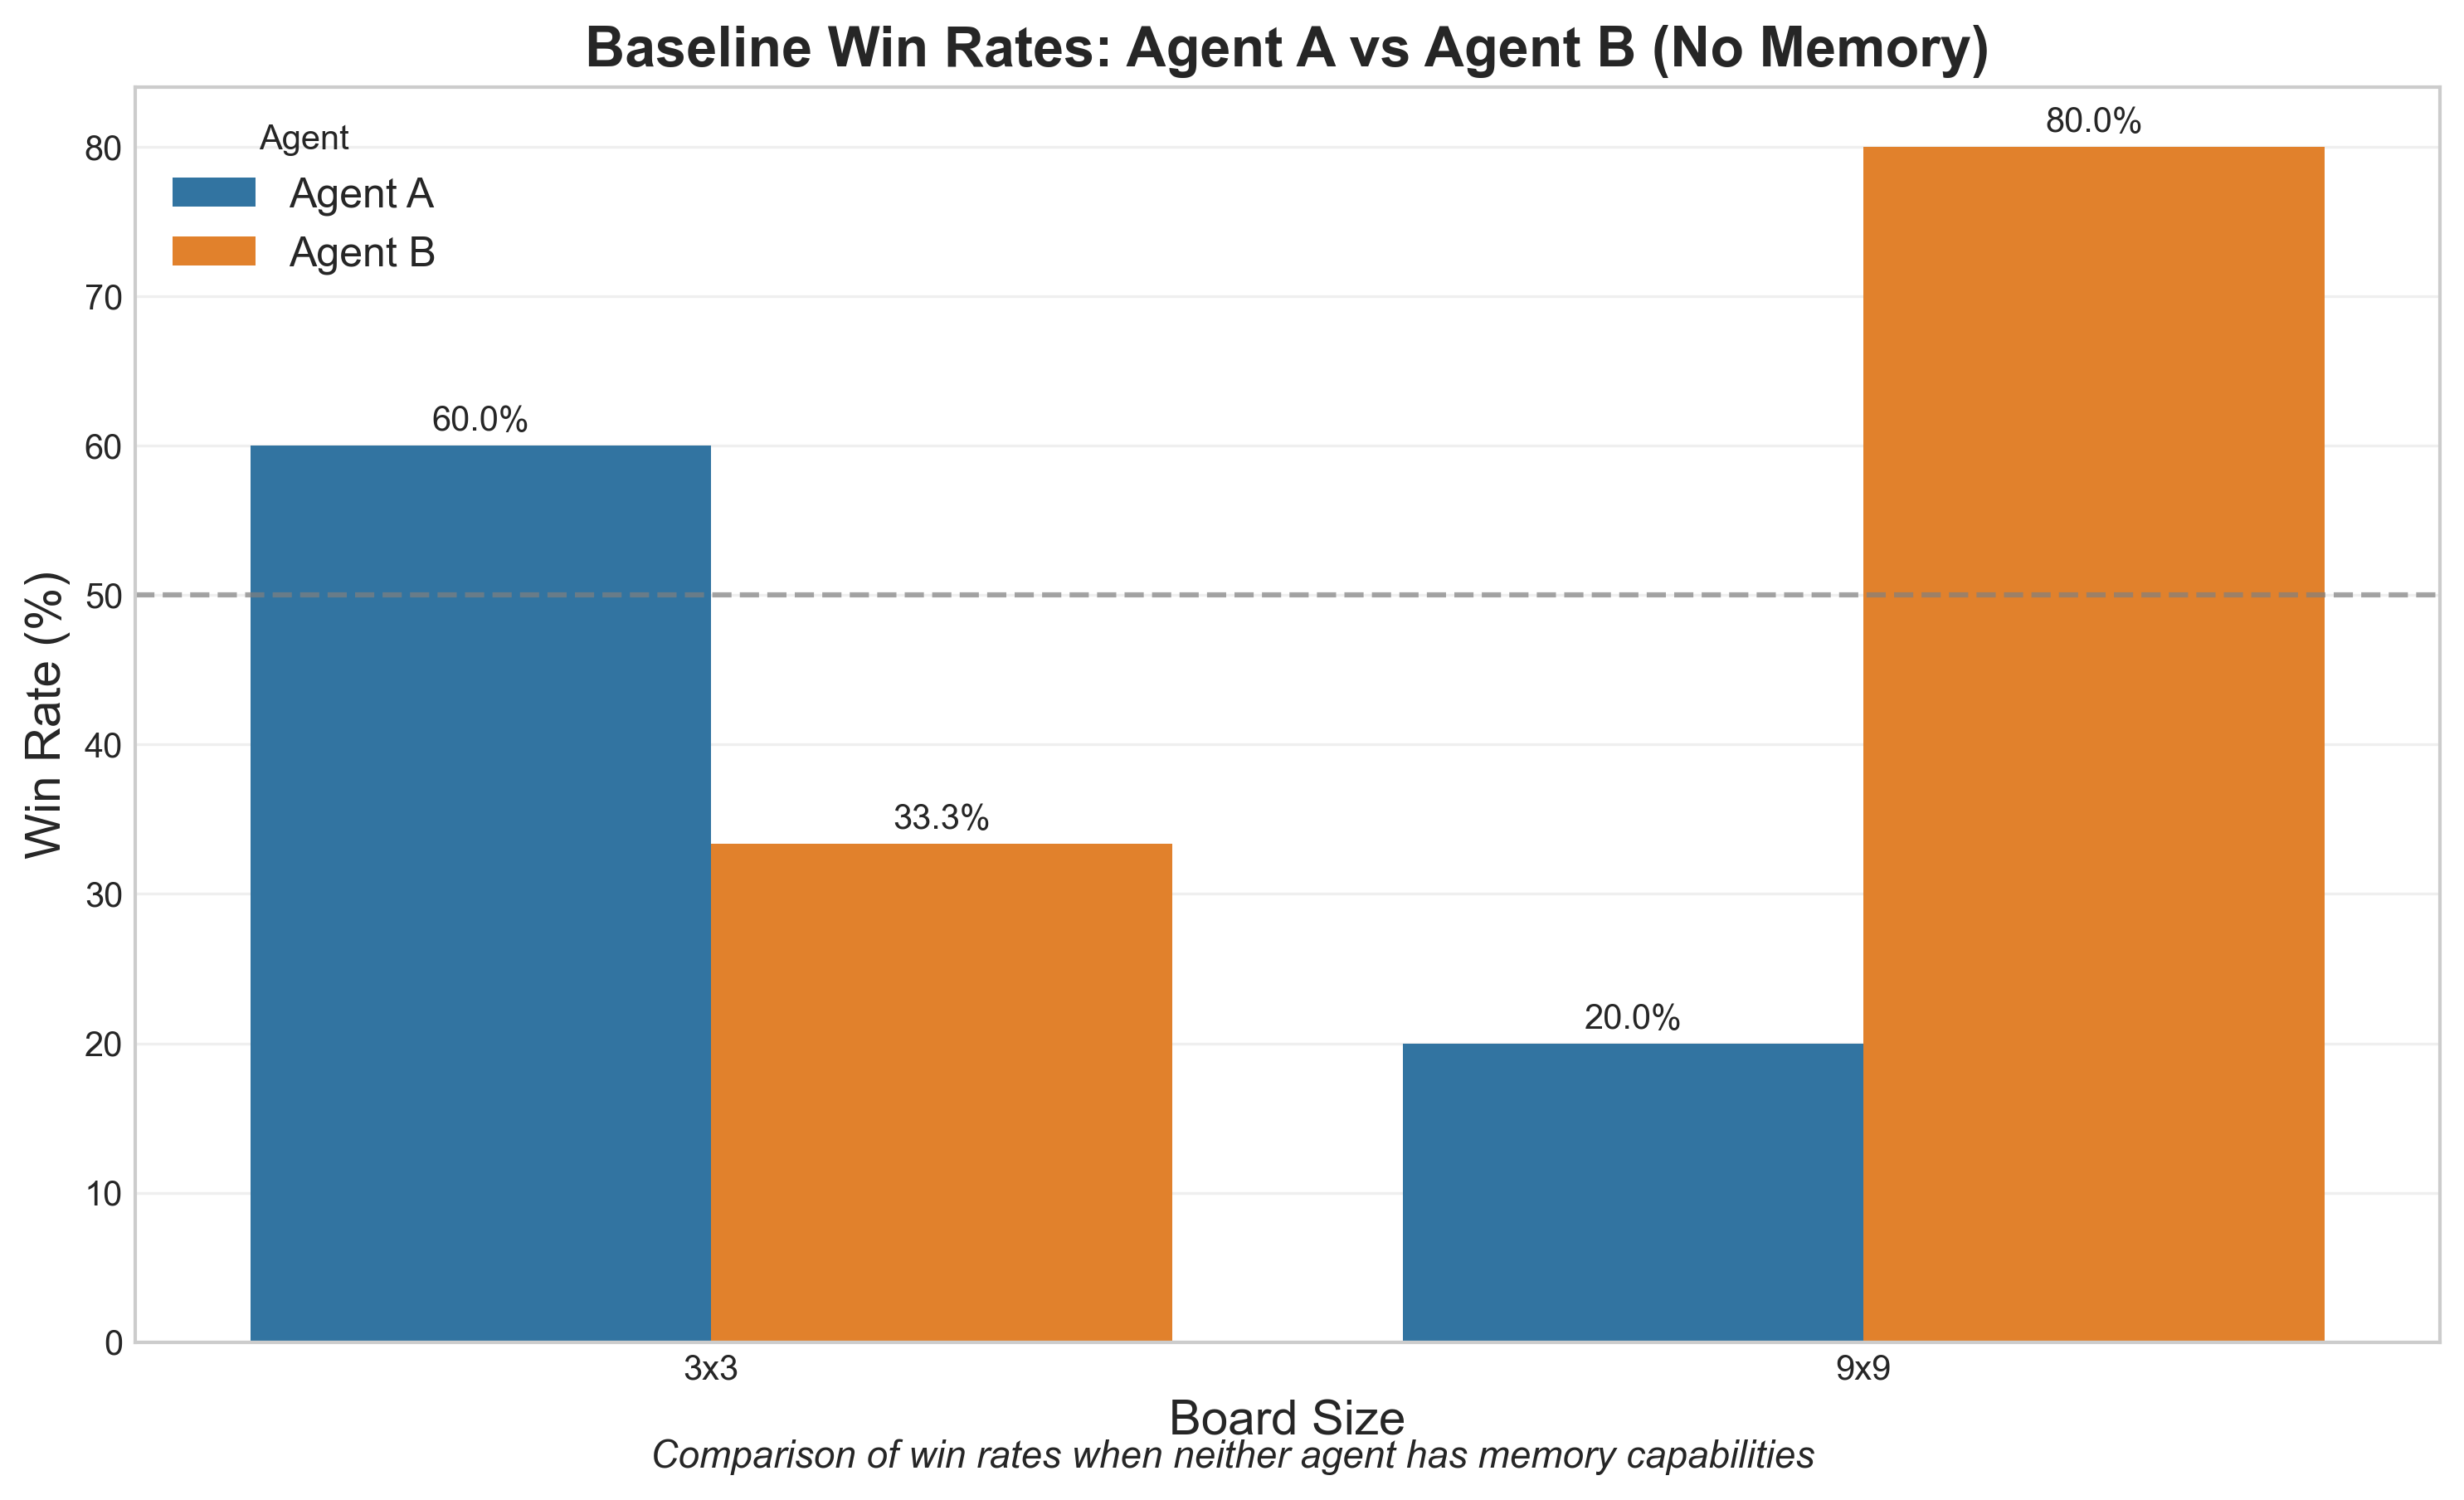
\includegraphics[width=0.6\textwidth]{figures/memory_baseline/baseline_win_rates.png}
\caption{Baseline win rates for Agent A and Agent B across board sizes (no memory).}
\label{fig:baseline_win_rates}
\end{figure}

To further illustrate the importance of memory augmentation, we compare each agent’s performance with and without memory. As shown in Figure~2, memory-augmented agents generally outperform their no-memory counterparts across both GraphMemory and VectorMemory settings, especially in smaller board environments ($3\times3$) where memory retrieval remains lightweight. This performance lift confirms that external memory helps stabilize reasoning and mitigate LLM struggles in complex decision-making.

However, for Agent A on $9\times9$ boards, this trend reverses: with-memory performance lags behind no-memory baselines. This counterintuitive result reflects both design logic and data-level factors. Agent A, driven solely by win maximization, tends to adopt aggressive memory usage patterns. While this strategy benefits from fast, similarity-based retrieval in VectorMemory, it suffers under GraphMemory’s relational overhead in large state spaces, where token costs and retrieval complexity increase. Since the aggregated results in Figure~2 combine both memory architectures, GraphMemory’s performance bottleneck drags down overall with-memory outcomes for Agent A at scale.

This highlights a critical insight: memory augmentation alone is insufficient without appropriate architectural choices. Effective memory strategies must balance retrieval efficiency and task complexity, particularly for aggressive agents operating under resource-intensive conditions.

\begin{figure}[H]
\centering
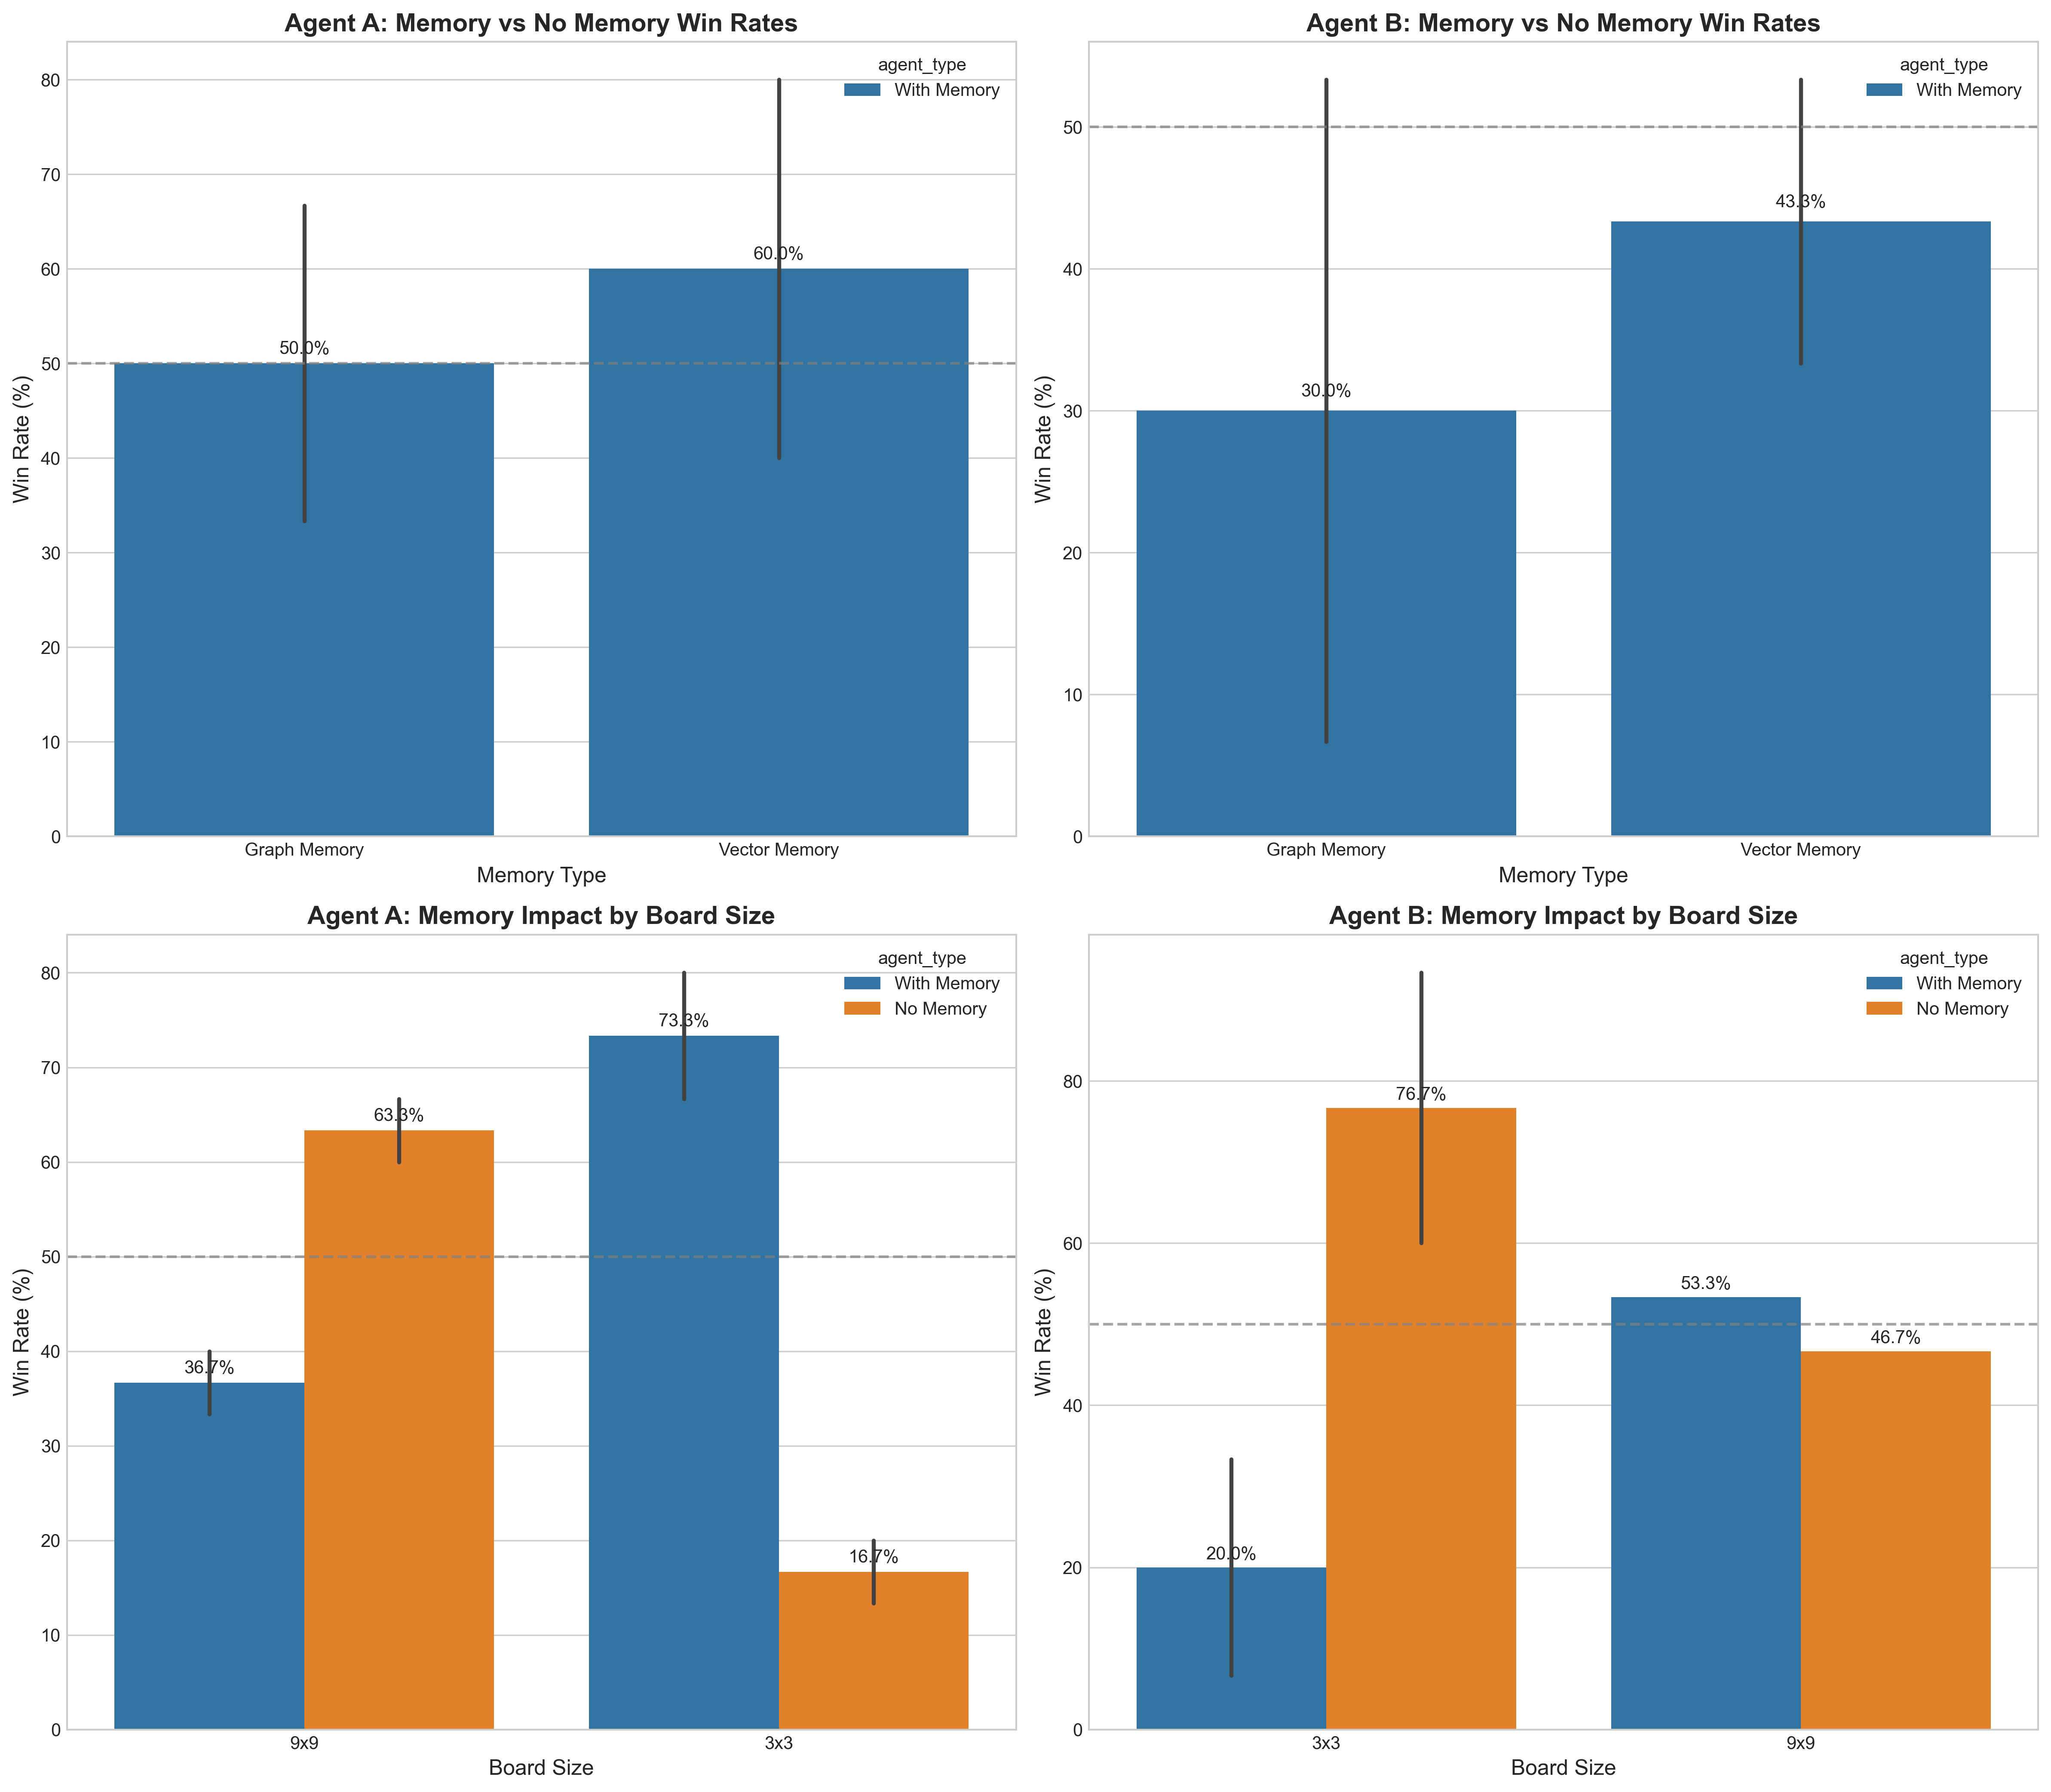
\includegraphics[width=0.7\textwidth]{figures/memory_baseline/memory_baseline_comparison.png}
\caption{Performance comparison within each agent: win rates with and without memory. Memory augmentation provides clear benefits across memory types and board sizes.}
\label{fig:memory_baseline_comparison}
\end{figure}

These findings establish two key points: 
\begin{enumerate}[leftmargin=*,nosep]
    \item Token-conscious prompting (Agent B) incurs a performance penalty in simple settings but enhances scalability in complex ones.
    \item External memory is likely critical for maintaining reasoning efficiency as task complexity grows.
\end{enumerate}

\subsection{Constrained Memory Experiments}

\subsubsection{RQ1: Memory Architecture Effectiveness}

To assess how different memory architectures influence performance, we compare GraphMemory and VectorMemory under constrained conditions, where agents are restricted to a single memory type. Table~\ref{tab:winrates} reports win rates for both agents across board sizes and memory types.

\begin{table}[h]
\centering
\small
\caption{Win rates across constrained memory types and board sizes.}
\begin{tabular}{@{}llcc@{}}
\toprule
Board Size & Memory Type & Agent A Win Rate & Agent B Win Rate \\
\midrule
$3\times3$ & Graph & 60.0\% & 20.0\% \\
$6\times6$ & Graph & 46.7\% & 53.3\% \\
$9\times9$ & Graph & 26.7\% & 73.3\% \\
\addlinespace
$3\times3$ & Vector & 66.7\% & 6.7\% \\
$6\times6$ & Vector & 60.0\% & 40.0\% \\
$9\times9$ & Vector & 53.3\% & 46.7\% \\
\bottomrule
\end{tabular}
\label{tab:winrates}
\end{table}

GraphMemory supports competitive performance on small boards, with Agent A achieving a \textbf{60.0\%} win rate on $3\times3$. However, as board size increases, GraphMemory's performance degrades significantly, with Agent A's win rate dropping to \textbf{26.7\%} on $9\times9$. Conversely, VectorMemory maintains more stable performance, with Agent A achieving \textbf{53.3\%} win rate on $9\times9$. This pattern supports \textbf{H1.2}, suggesting that VectorMemory's similarity-based retrieval scales more effectively as the state space expands.

\textbf{Figure Placeholder}: Performance retention analysis (normalized win rates relative to $3\times3$).

Retention plots reveal that VectorMemory preserves roughly \textbf{80\%} of its baseline performance on $9\times9$, while GraphMemory retention falls below \textbf{50\%}. These results confirm that memory architecture directly impacts scalability and decision quality, particularly in complex environments.

\subsubsection{RQ2: Memory Usage Growth with Complexity}

To investigate how memory usage scales with task complexity, we track the number of memory function calls per game across agents, memory types, and board sizes.

VectorMemory usage exhibits a \textbf{monotonic increase} in memory calls as board size grows, with Agent A's calls rising from \textbf{4} on $3\times3$ to \textbf{20} on $9\times9$. GraphMemory, in contrast, shows \textbf{non-linear growth}: memory calls peak at $6\times6$ (\textbf{21} calls for Agent A) but drop on $9\times9$ (\textbf{12} calls). This irregular pattern suggests diminishing returns from GraphMemory in larger, less structured state spaces.

Agent A consistently makes \textbf{2--4 times more memory calls} than Agent B, reinforcing \textbf{H3.1} that win-maximizing agents are more liberal in memory usage. Agent B, constrained by token efficiency, remains more conservative.

\textbf{Figure Placeholder}: Memory calls by board size and memory type.

These findings align with \textbf{H2.1} and \textbf{H2.2}, indicating that memory demand grows with complexity but is mediated by both architecture and agent objective.

\subsection{RQ3: Memory Quantity $\neq$ Performance}

To investigate whether higher memory usage directly correlates with better performance, we plot \textbf{total memory calls per game} against \textbf{win rate} across all constrained memory conditions (Figure~\ref{fig:memory_quantity_performance}). Each point represents one agent-memory-board configuration.

\begin{figure}[ht]
\centering
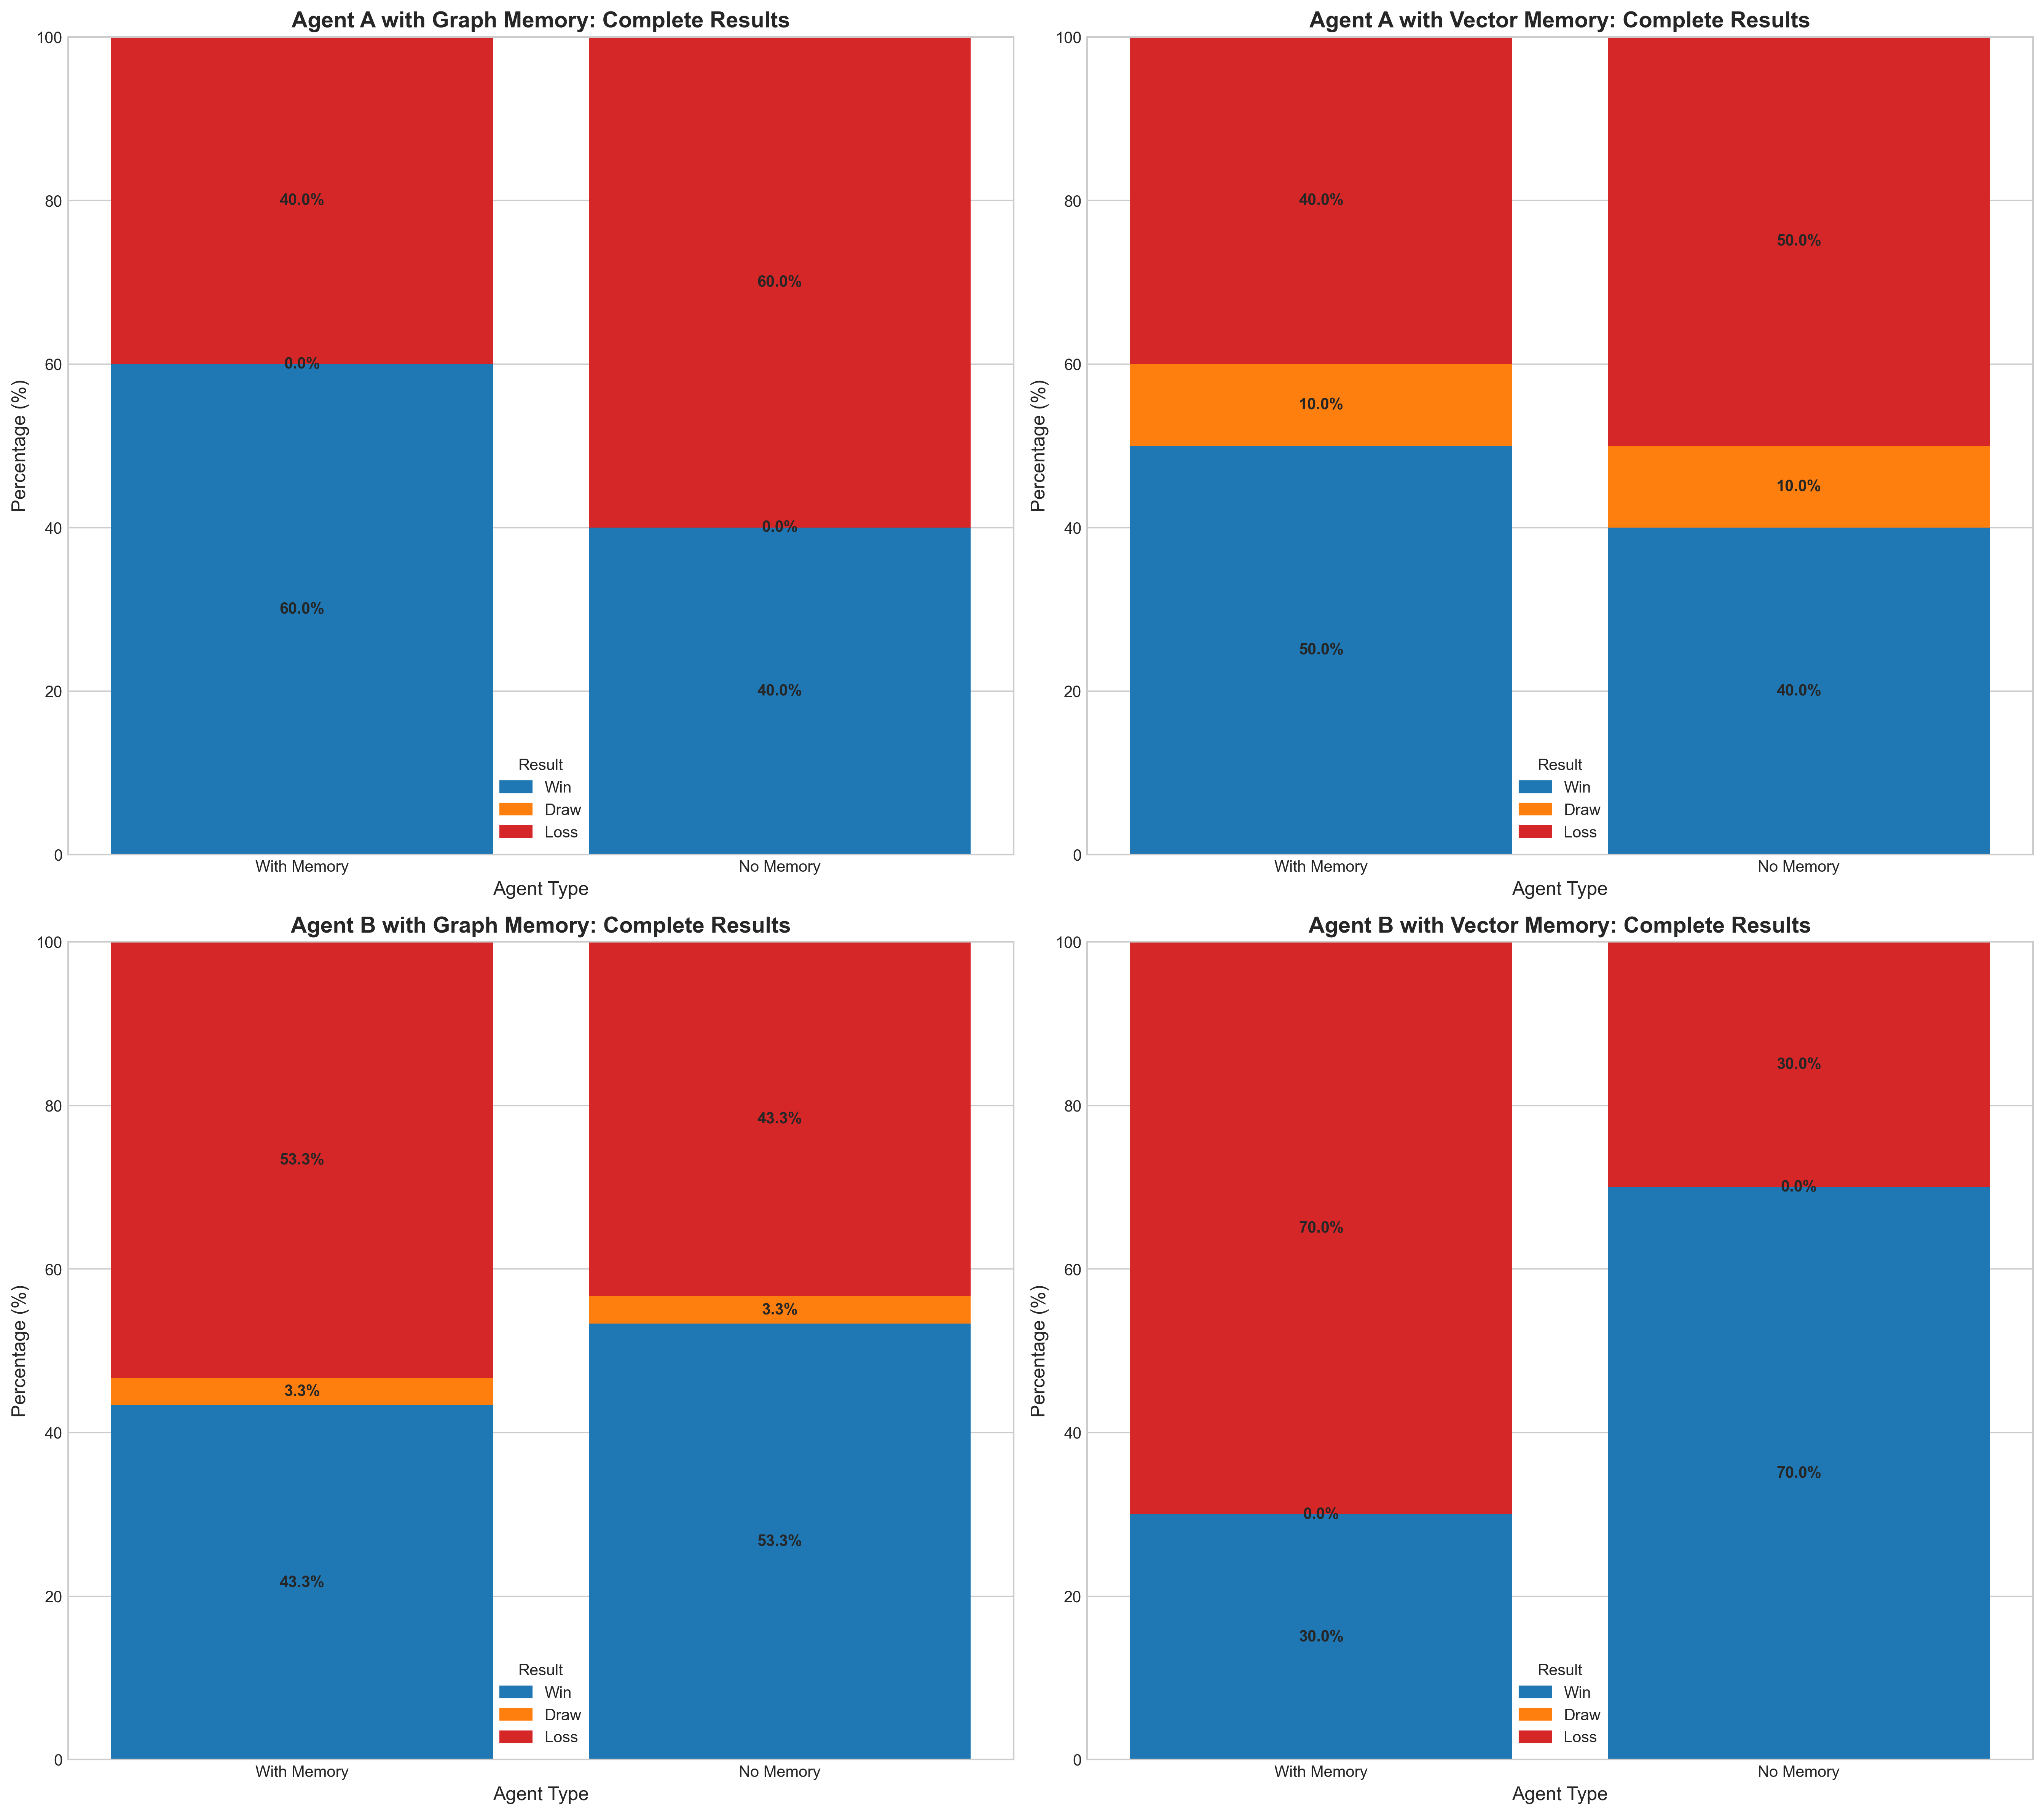
\includegraphics[width=0.55\textwidth]{figures/memory_baseline/memory_complete_results.png}
\caption{Win rate vs. total memory calls across constrained settings. Agent A (blue) consistently calls memory more often than Agent B (orange).}
\label{fig:memory_quantity_performance}
\end{figure}

This analysis reveals two key patterns. First, \textbf{Agent A consistently makes more memory calls} than Agent B across all conditions---often 2--4 times more. This aligns with their respective prompt framings: Agent A operates under pure win maximization, whereas Agent B accounts for token efficiency.

However, \textbf{more memory calls do not guarantee better performance}. In fact, some of Agent A's highest memory-call configurations (e.g., GraphMemory at $6\times6$) correspond to \textbf{only moderate win rates} (around 46.7\%). This suggests diminishing returns: aggressive memory use may saturate, leading to noisy or redundant retrievals that do not significantly improve decision quality.

Conversely, Agent B achieves \textbf{competitive or superior win rates with fewer memory calls}---particularly in larger board settings like $9\times9$. This selective behavior reflects its internalization of token cost constraints and supports the broader finding that \textbf{memory quality matters more than quantity}. 

In sum, RQ3 is supported: \textbf{memory quantity alone is not a reliable predictor of agent success}. Instead, strategic timing and relevance of memory access shape performance outcomes.

\subsection{RQ4: Memory Efficiency Tradeoff}

We further explore the \textbf{efficiency of memory usage} by analyzing \textbf{win rate-to-token ratios} across board sizes for both agents (Figure~\ref{fig:memory_efficiency_tradeoff}). This metric captures the \textbf{strategic value per token spent}.

\begin{figure}[ht]
\centering
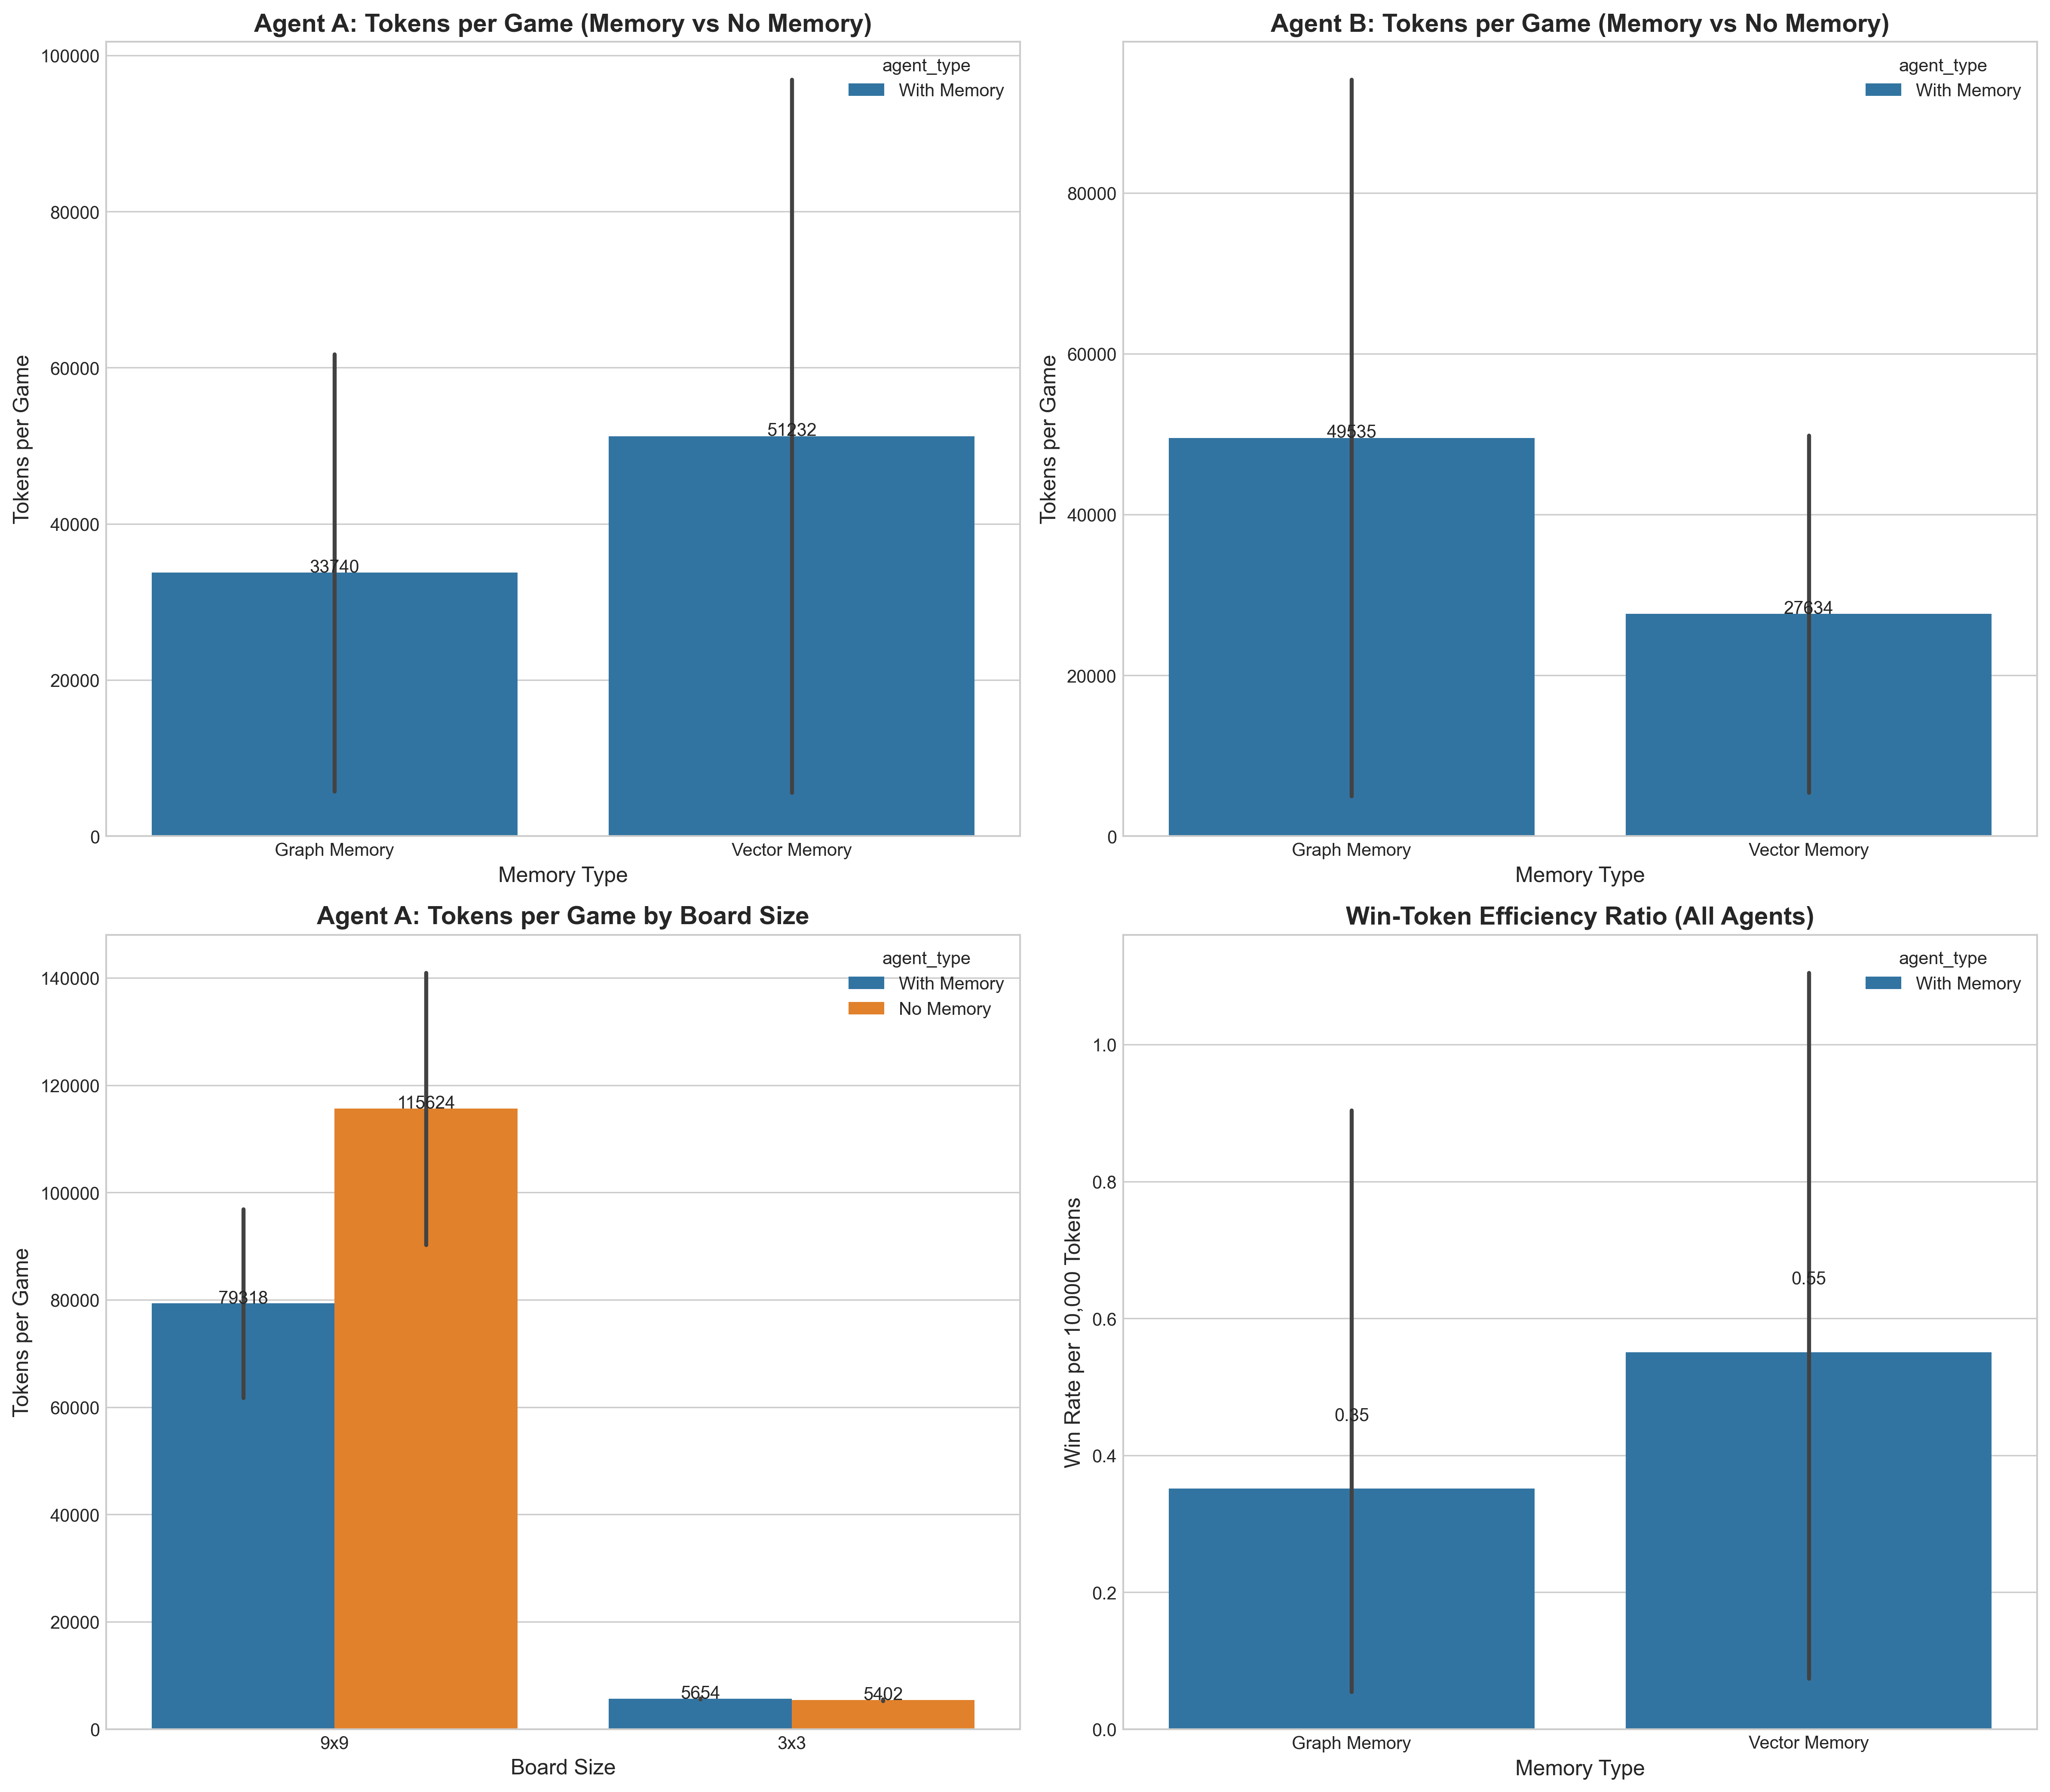
\includegraphics[width=0.55\textwidth]{figures/memory_baseline/memory_token_efficiency.png}
\caption{Win rate-to-token ratio by agent and board size. Higher values indicate greater efficiency.}
\label{fig:memory_efficiency_tradeoff}
\end{figure}

Three clear trends emerge. First, \textbf{Agent A exhibits high efficiency on $3\times3$ boards}, largely due to minimal token overhead in a simple environment. However, as board complexity increases, \textbf{Agent A's efficiency deteriorates sharply}, dropping to \textbf{0.08} on $9\times9$ boards. This reflects its aggressive, unfiltered memory usage---retrieving often without regard to computational cost.

In contrast, \textbf{Agent B maintains relatively stable efficiency across board sizes}, despite lower raw win rates. This stability arises from \textbf{fewer but more deliberate memory calls}, reflecting its cost-sensitive strategy. Even in the most complex environment ($9\times9$), Agent B sustains \textbf{efficiency levels multiple times higher} than Agent A.

These results validate \textbf{H3.2}, confirming that \textbf{objective-aligned memory strategies emerge}. While Agent A prioritizes victory at any cost, Agent B adapts to balance performance with resource constraints---demonstrating \textbf{more disciplined, scalable memory usage}.

Taken together, RQ4 supports the conclusion that \textbf{agent objectives directly shape memory efficiency tradeoffs}, with token-conscious agents exhibiting greater resilience in resource-constrained settings.

\subsection{RQ5: Adaptive Memory Experiments}

In the adaptive setting, agents were granted full access to all memory types—GraphMemory, VectorMemory, and SemanticMemory (though the latter remained largely unused). This experiment aimed to investigate whether agents could autonomously learn not only \textbf{when} to engage memory, but also \textbf{which} memory type to select, depending on task complexity and internal objectives.

\paragraph{Memory Type Preferences.}  
Our first observation centers on \textbf{memory type selection patterns} across board sizes. Figure~\ref{fig:adaptive_memory_type} presents the distribution of memory type usage for each agent. As hypothesized, both agents demonstrated a marked preference for \textbf{VectorMemory} on larger boards ($6\times6$ and $9\times9$), aligning with the results from constrained experiments. Specifically, VectorMemory accounted for over \textbf{70\%} of memory calls in $9\times9$ games for both agents.

GraphMemory was used sporadically, primarily on smaller boards, while SemanticMemory remained essentially unused, reflecting its placeholder implementation in this iteration. On the simplest board ($3\times3$), \textbf{Agent A made no memory calls}, while Agent B engaged memory on approximately \textbf{13\% of turns}, selectively invoking it when efficiency outweighed cost.

\paragraph{Memory Call Frequency.}  
Figure~\ref{fig:adaptive_memory_frequency} shows the \textbf{average memory calls per game} in adaptive mode. Compared to constrained settings, where memory use increased significantly with board size, adaptive agents exhibited \textbf{far sparser memory engagement}. This difference was most pronounced for \textbf{Agent B}, which consistently minimized memory use, especially on smaller boards.

Interestingly, even as board complexity grew, agents maintained a relatively \textbf{flat memory call profile}, indicating deliberate, selective use. This contrasts with the more aggressive, architecture-driven memory patterns seen in constrained experiments, suggesting that when afforded choice, agents regulate memory more tightly.

\paragraph{Token Usage and Efficiency.}  
Token efficiency patterns mirrored memory behavior. Figure~\ref{fig:adaptive_token_efficiency} compares the \textbf{win-rate-to-token ratio} across board sizes for both agents in adaptive mode. Agent B once again demonstrated superior efficiency, maintaining \textbf{lower token consumption per win} than Agent A, particularly on \textbf{$9\times9$ boards}.

Crucially, Agent B's token usage in adaptive mode was \textbf{even lower} than in constrained settings, highlighting the benefits of flexible memory selection. This finding reinforces our hypothesis that \textbf{agents learn to balance performance and cost dynamically} when given the freedom to choose memory types.

\paragraph{Performance Tradeoffs.}  
Despite its more conservative memory usage, Agent B's performance remained competitive. Figure~\ref{fig:adaptive_performance_tradeoff} plots \textbf{win rate versus token usage} for both agents. Agent A consistently achieved higher win rates, particularly on larger boards, but at the cost of significantly higher token consumption. Agent B, while accepting a modest drop in win rate, achieved a superior \textbf{win-token tradeoff}, underscoring the effectiveness of its resource-aware strategy.

These findings support \textbf{H4} and \textbf{H5}, demonstrating that:
\begin{enumerate}[leftmargin=*,nosep]
    \item Agents can autonomously adapt memory usage frequency and type selection to context;
    \item Token-efficient agents (Agent B) leverage this flexibility to optimize resource allocation without sacrificing competitive performance.
\end{enumerate}

\paragraph{Summary.}  
The adaptive experiments reveal that when freed from architectural constraints, agents develop distinct memory strategies that align with their objectives. VectorMemory remains the dominant choice at scale, but memory usage overall becomes more selective, leading to improved token efficiency, particularly for cost-aware agents. This adaptability suggests that LLM agents can internalize complex tradeoffs between performance and efficiency, tuning both memory engagement and architecture preference dynamically.

\begin{figure}[ht]
\centering
% \includegraphics[width=0.48\textwidth]{adaptive_memory_type.png}
\caption{Memory type distribution across board sizes in adaptive mode. VectorMemory dominates on larger boards.}
\label{fig:adaptive_memory_type}
\end{figure}

\begin{figure}[ht]
\centering
% \includegraphics[width=0.48\textwidth]{adaptive_memory_frequency.png}
\caption{Average memory calls per game: adaptive vs. constrained modes.}
\label{fig:adaptive_memory_frequency}
\end{figure}

\begin{figure}[ht]
\centering
% \includegraphics[width=0.48\textwidth]{adaptive_token_efficiency.png}
\caption{Win rate-to-token ratio in adaptive mode across board sizes.}
\label{fig:adaptive_token_efficiency}
\end{figure}

\begin{figure}[ht]
\centering
% \includegraphics[width=0.48\textwidth]{adaptive_performance_tradeoff.png}
\caption{Win rate vs. token usage for both agents in adaptive mode.}
\label{fig:adaptive_performance_tradeoff}
\end{figure}

\section{Discussion}

\subsection{Implications for Memory Architecture Design}

Our findings carry several implications for the design of memory systems in LLM agents. First, the consistent superiority of \textbf{VectorMemory} across increasing task complexity suggests that \textbf{fuzzy retrieval mechanisms} generalize more effectively than structured, relational storage in high-variance environments. While \textbf{GraphMemory} offers clear benefits in smaller, well-structured settings (e.g., the $3 \times 3$ board), its performance degrades sharply as the environment scales. This indicates that graph-based relational reasoning—while interpretable—faces scalability limits when the number of potential state transitions explodes. In contrast, the pattern-matching capabilities of vector-based retrieval, powered by latent-space embeddings, allow agents to flexibly navigate large and sparsely populated state spaces. This suggests that for agents operating in open-ended or poorly structured environments, \textbf{vector-based memory architectures may offer more robust scalability}, a principle likely to extend beyond TicTacToe.

Second, our experiments highlight the subtle but significant influence of \textbf{prompt framing} in shaping agent behavior, even when optimization objectives remain formally identical. Though both agents were tasked with maximizing win rate while minimizing token use, Agent B's repeated reminders about token costs led to \textbf{emergent resource-conscious strategies}—characterized by lower memory usage frequency and greater token efficiency. This divergence demonstrates that \textbf{prompt design acts as a soft constraint} on LLM agents, shaping not only local decision-making but broader strategic patterns over time. For developers of cognitive architectures and LLM-based planning agents, this finding underscores the need to carefully craft system-level prompts, as these seemingly minor choices can have outsized effects on agent behavior.

Finally, the tradeoff between \textbf{aggressiveness} and \textbf{efficiency} that emerged across our agents offers further insights for LLM-based agent design. Agent A's strategy—driven solely by win maximization—led to more frequent memory use, but with diminishing returns at scale. Agent B, by contrast, balanced token costs and selectively used memory, yielding \textbf{better performance retention} and \textbf{higher win-rate-to-token ratios} in larger environments. This suggests that, especially in resource-constrained settings, \textbf{conservative memory strategies} may support more scalable and robust agent performance.

\subsection{Limitations and Reflection}

While our results offer valuable insights, they are bounded by several limitations. First, our experiments are confined to the domain of TicTacToe, albeit scaled up to larger boards. Though this scaling increases complexity, the task remains relatively simple and deterministic. More complex environments—such as Connect4 or open-ended dialogue planning—may introduce dynamics that challenge the current memory architectures differently.

Second, our implementation of \textbf{SemanticMemory} remains incomplete. Though conceptually included as a third modality for higher-level strategy storage, it was not evaluated in these experiments. The absence of this modality limits our conclusions about how agents might select among richer memory types in adaptive settings. Additionally, our evaluation of \textbf{adaptive memory selection} was limited by sample size, leading to noisier trends and inconclusive results about how agents might balance memory type selection in open-choice conditions.

Third, our agents operated under a fixed \textbf{token tradeoff parameter} ($\lambda$). While we observed clear differences in behavior between Agent A ($\lambda = 0$) and Agent B (explicit token cost framing), we did not explore how varying $\lambda$ dynamically might affect strategy adaptation. Real-world systems may benefit from flexible tradeoff adjustments, especially in resource-bounded environments.

Finally, while our memory operations—\texttt{store}, \texttt{retrieve}, and \texttt{update schema}—support basic episodic retrieval, they do not model more advanced mechanisms such as \textbf{memory compression}, \textbf{schema evolution}, or \textbf{long-term forgetting}. Our logs indicate that schema updates were rare, suggesting that \textbf{meta-memory reasoning} was underutilized in this setup. Future systems might benefit from richer forms of memory management, including learned compression strategies or explicit schema optimization.

\subsection{Future Directions}

Our study suggests several promising avenues for further research. First, extending the environment to \textbf{longer-horizon tasks}—such as Connect4 or multi-step planning domains—would better test the limits of memory scalability and generalization. Second, exploring \textbf{dynamic $\lambda$ tuning}—potentially allowing agents to adjust their efficiency-performance tradeoff over time—could reveal more adaptive behaviors. Third, completing and integrating \textbf{SemanticMemory} would enable full evaluation of adaptive memory selection, testing whether agents can learn to balance structured, fuzzy, and conceptual storage systems depending on context.

Finally, incorporating \textbf{reinforcement learning} to explicitly train agents not just on task objectives but on memory usage patterns—such as when to update schemas or compress memories—could foster richer, more efficient memory behaviors. Such extensions would move beyond static prompting, enabling agents to learn \textbf{meta-strategies} for memory management over time.

\section{Conclusion}

This study explored how LLM agents equipped with modular external memory systems develop usage strategies under differing objectives and environmental complexities. By embedding GPT-4o-mini agents in self-play TicTacToe games across board sizes, and equipping them with \textbf{GraphMemory} and \textbf{VectorMemory}, we systematically investigated how memory architecture and prompt framing shape agent behavior. Our experiments reveal that:

\begin{itemize}[leftmargin=*,nosep]
    \item \textbf{VectorMemory scales more robustly} across increasing board sizes, outperforming GraphMemory in large, sparse state spaces.
    \item \textbf{Agent objectives significantly influence memory usage}, with token-aware agents demonstrating more selective and efficient memory strategies, despite identical formal optimization goals.
    \item \textbf{More memory does not always translate to better performance}; rather, targeted, efficient memory use—particularly under resource constraints—supports better scalability.
\end{itemize}

These findings contribute to a growing understanding of how \textbf{adaptive memory systems} can support LLM-based agents in complex, sequential reasoning tasks. They emphasize that both \textbf{memory architecture} and \textbf{prompt design} play critical roles in shaping agent behaviors, extending beyond the raw capabilities of the underlying LLM.

Looking forward, this work opens pathways for richer memory models and more adaptive agent designs. Integrating diverse memory systems (structured, fuzzy, semantic) and developing meta-learning strategies for memory management could unlock new capabilities in LLM agents, making them more effective, scalable, and efficient across a broad range of domains.

% Fix for bibliography processing
\bibliographystyle{plainnat}
\bibliography{bibliography}

\end{document}
